\documentclass[12pt]{article}
\usepackage[utf8x]{inputenc}
\usepackage[colorinlistoftodos]{todonotes}
\usepackage[bookmarks=true]{hyperref}
\usepackage{float}
\usepackage{placeins}
\usepackage{listings}
\usepackage{enumitem}
\usepackage{marvosym}
\usepackage{lmodern,textcomp}
\usepackage{amsmath}
\usepackage{algorithm}
\usepackage{algorithmic}

\hypersetup{pdftitle={Princing And Advertising},
	pdfauthor={Andrea Furlan, Cosimo Russo, Giorgio Ughini},        
	pdfsubject={DIA},
	colorlinks=true,
	linkcolor=blue,
	citecolor=blue,
	filecolor=black
	urlcolor=purple,
}

\begin{document}
	\begin{titlepage}
		\newcommand{\HRule}{\rule{\linewidth}{0.7mm}}
		\center
		
\includegraphics{PolimiLogo.png}\\[1cm]
		
		\textsc{\LARGE Project Report Document}\\[1cm]
		\textsc{\large Data Intelligence Application - A.Y. 2019-2020}\\[1cm]
		\HRule \\[0.4cm]
		{ \huge \bfseries Pricing and Advertising}\\[0.15cm]
		\HRule \\[1.5cm]
		{\large Authors  \hfill ID Numbers}\\[0.4cm]
		{\large Andrea \textsc{Furlan}  \hfill 944774}\\[0.2cm]
		{\large Cosimo \textsc{Russo}  \hfill 945891}\\[0.2cm]
		{\large Giorgio \textsc{Ughini} \hfill 944710}\\[2cm]
		{\large \today  \hfill Version 1.0}
		\vfill
	\end{titlepage}
	\clearpage
	{\hypersetup{hidelinks}\tableofcontents}
	\clearpage
	\section{Introduction}
	\subsection{The Product}
	\begin{figure}[!htp] 
	\begin{flushleft}
		In this project we would like to focus our attention on a specific product: a luxury scarf. We decided to take into consideration this item because it's a seasonal product that is more searched by its buyers in the cold seasons and less demanded during the summer days. This periodic variation of the users' interests is an interesting input to take in consideration during our analysis. We decided to use as a subject the classical Louis Vuitton brand logo scarf, well known and trending in our country.
	\end{flushleft}
	\centering
	
\includegraphics[width=0.8\linewidth]{sections/productLogo}
	\caption{Louis Vuitton Brand Logo Scarf.}
\end{figure}
\clearpage
	\subsection{The Classes of Users}
	Given that the product we want to study generates more interest in women rether than in men, we decided to focus our studies on women only. We also came to the conclusion that since a luxury scarf is usually bought from the middle and the upper class person, a minimum family yearly income bound was necessary to set our focus on only the users that are able to generate more impact on the analysis. We set this bound at 80.000 \EUR{} gross. Finally we thought that since trends can vary among countries, considering only the Italian population was the most reasonable choice to avoid unwanted biases.
The binary features that we decided to observe on our users are:
\begin{itemize}
	\item \textbf{With/Without children}:\@ To better observe the impact that a son can have in buying a luxury item
	\item \textbf{Living in the North/South of Italy}:\@ To better observe the impact that the climate and the local traditions can have in buying an item that is useful only in certain seasons.
\end{itemize}
The distribution of our customer base is described in the following pie chart:
\makebox[\textwidth][c]{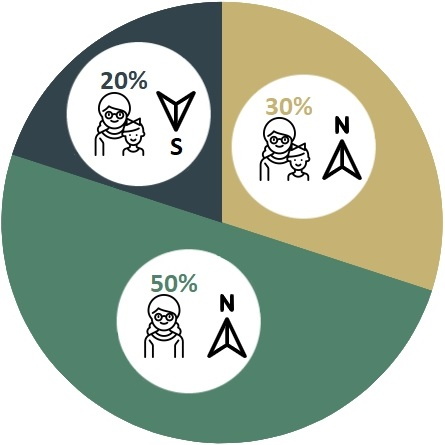
\includegraphics[width=0.7\textwidth]{sections/images/usersImage3}}
%\makebox[\textwidth][c]{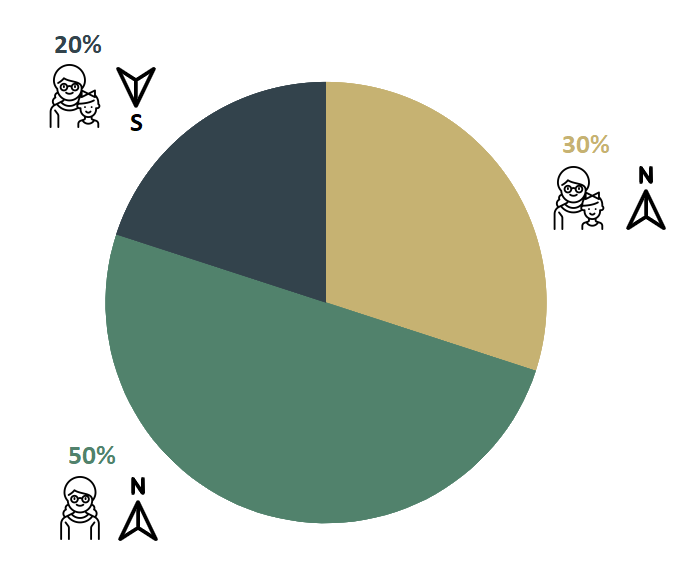
\includegraphics[width=0.9\textwidth]{sections/images/usersImage}}
	\subsection{The Conversion Rate Curves}
	Since the Louis Vuitton brand logo scarf is classified as a luxury good, we hypothesised the three conversion rate curves to have non-negative-slope and reaching their peak near the \EUR{200-250} range. \\These curves are the curves that rule the environment of our experiment.\\An illustration of our hypothesised conversion rate curve is presented below:\newline
\makebox[\textwidth][c]{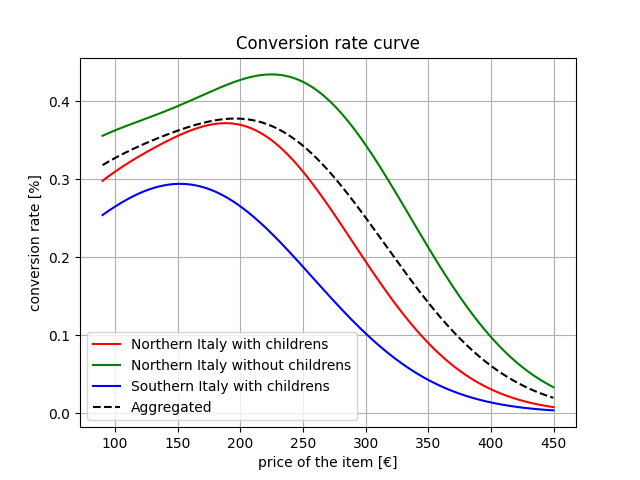
\includegraphics[width=1.1\textwidth]{../curves/real_curves/conversion_rate_curve}} 
\clearpage
	\subsection{The Subcampaigns}
	In order to advertise our product we outlined three different sub-campaign each with a unique aspect and a particular type of user as a target. The three sub-campaigns are focused on:
\begin{itemize}
	\item \textbf{The Quality Of The Product}:\@ \newline Targeting the women with children living in the north of Italy.
	\item \textbf{The Social Impact Generated By The Product}:\@ \newline Targeting the women without children living in the north of Italy.
	\item \textbf{The Peculiarity And The Uniqueness Of The Product}:\@ \newline Targeting the women with children living in the south of Italy.
\end{itemize} 
An idea of how the ads could be is the following: \newline\\\\
\makebox[\textwidth][c]{
\includegraphics[width=1.2\textwidth]{sections/images/ad1}}
\makebox[\textwidth][c]{
\includegraphics[width=1.2\textwidth]{sections/images/ad2}}
\makebox[\textwidth][c]{
\includegraphics[width=1.2\textwidth]{sections/images/ad3}}

	\subsection{The Abrupt Phases}
	As we said in the first section, the product taken into analysis is a seasonal item. Using Google Trends, we were able to identify the region of maximum and minimum interest of the users regarding a Louis Vuitton scarf. In the graph below is clear that this product is searched primarily in the cold seasons and it is year after year more demanded by the customers. In the chart the x-axis represents a five year time period while the y-axis represents the popularity of the keywords "Louis Vuitton Scarf" searched on Google (100 is the moment of maximum interest while 0 is the minimum).
\makebox[\textwidth][c]{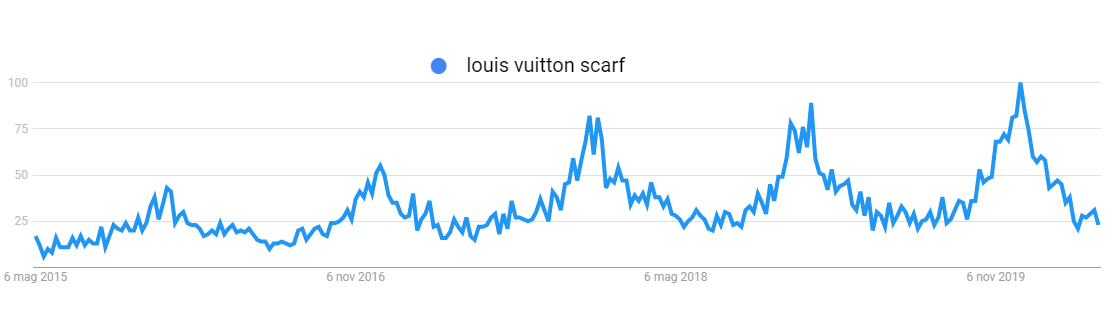
\includegraphics[width=1.2\textwidth]{sections/images/trend}}
Based on the diagram we decided to divide the year in four periods of time, each one underlining a different phase.\newline\\
\makebox[\textwidth][c]{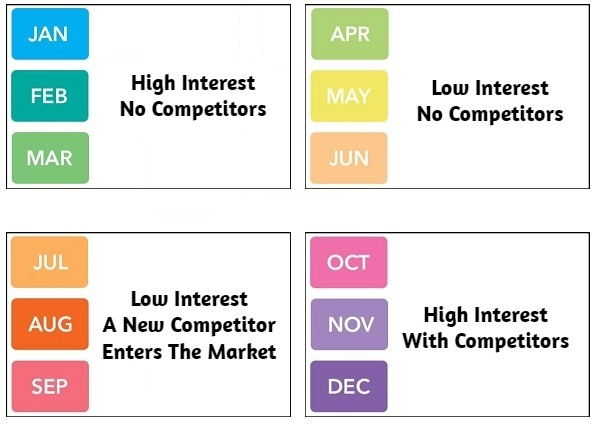
\includegraphics[width=0.8\textwidth]{sections/images/months}}
In order to better understand our reasoning behind the decisions that brought us to choose as graphs for the four different phases the ones showed below, is important to notice some remarks. \\In the first phase (Jan-Feb-Mar) the growth of the curve is almost linear, since there are no competitors that can interfere with our advertising of the product, but still there is a large pool of users to influence, since it is a phase of high interest of the product.\\ In the second phase (Apr-May-Jun) instead, since in these months the interest about the item is low, there will be less people interest in the scarf, therefore the impact that a higher budget allocated to the ads can make is less relevant that the impact that it can produce on a high interest phase. Based on this assumption we decided that the graph for the second phase should have a more remarkable growth with a small budget allocated to the ads, settling to much more slower growth as the budget significantly increases. \\In the next phase (Jul-Aug-Sep), when the new competitor enters the market, the graph should be different in the low budget allocated range respect to the second graph, while maintaining a similar profile in the high budget allocated range. The cause is the following: since we need to beat the competition in order to sell our product, we will struggle to do so allocating a small amount of money to the advertisement, while instead allocating a sufficient amount of money, we should be able to attract user to us as if there was not a competitor in the market. \\Finally, in the last phase (Oct-Nov-Dec) we focussed on the fact that since it is an high interest phase, but this time with a competitor that challenges us, the budget that needs to be allocated to the sub-campaigns still needs to be a considerable amount if we want to attract a sufficient number of users as in the third phase, but in this period the pool of users that can be reached is much wider, translating in a more linear curve in the high budget allocated range with respect to the third phase.\\
Taken into consideration our reasoning, the images below will present the structure of the probability distribution over the daily number of clicks for every value of budget allocated to that sub-campaign.\\
\makebox[\textwidth][c]{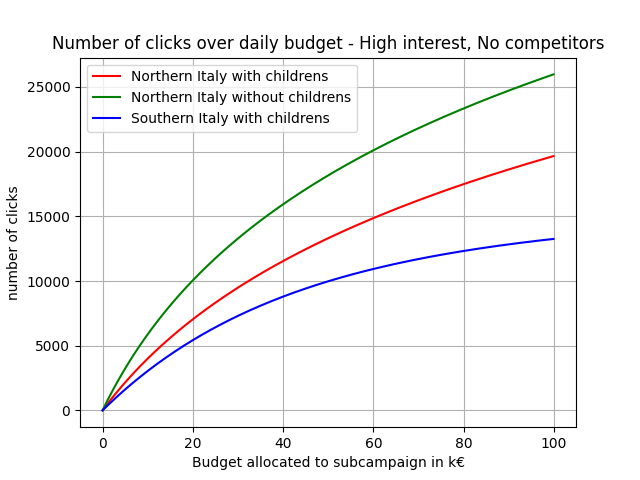
\includegraphics[width=0.85\textwidth]{../curves/real_curves/daily_clicks_10}} 
\makebox[\textwidth][c]{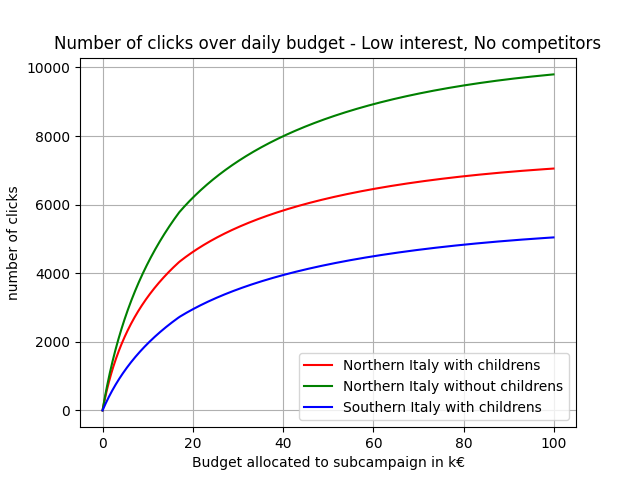
\includegraphics[width=0.85\textwidth]{../curves/real_curves/daily_clicks_00}} 
\makebox[\textwidth][c]{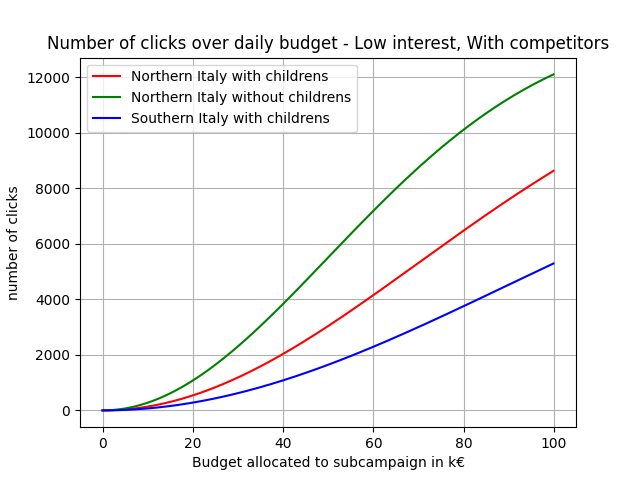
\includegraphics[width=0.85\textwidth]{../curves/real_curves/daily_clicks_01}} 
\newline\\\\
\makebox[\textwidth][c]{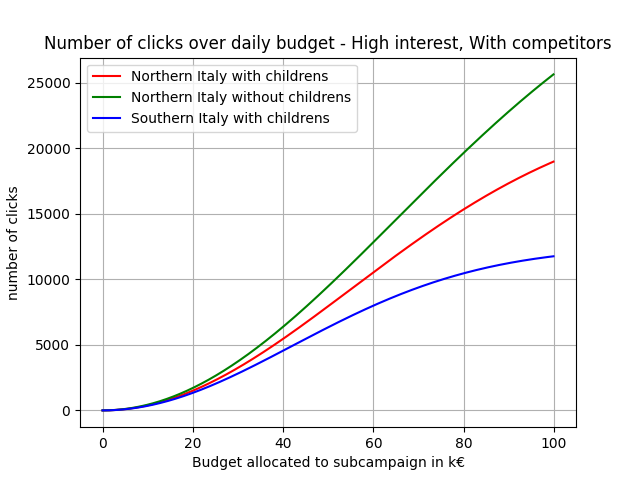
\includegraphics[width=0.85\textwidth]{../curves/real_curves/daily_clicks_11}} 
	\section{Case study and Algorithms}
	\subsection{Budget allocation with only one phase}
	The first step of our project was focused on the budget allocation over the three subcampaigns and had as goal the maximization of the total number of clicks.
In this first stage, for simplicity, only one phase is considered.
	\subsubsection{Experiment setting}
	The first step of the process is the definition of the size of the experiments, in particular:
\begin{itemize}
	\item \textbf{The number of arms}:\@  the higher it is, the more likely is the chance of exploring
	arms that are close to the optimal arm. On the other hand, having more arms
	implies that the optimization horizon will be required to be longer to allow a
	proper exploration of all the arms.
	\item \textbf{The optimization horizon}:\@  this is the amount of time that will be spent
	running the price optimization algorithms. The longer this is, the more are
	the possibilities that can be explored. However, exploring more possibilities
	causes to have a bigger loss - or regret - in the initial phases of the exploration.
\end{itemize} 
It appears clear that the the two quantities depend one on each other
and represent the key of the optimization. A reasonable optimization horizon is
one year. Indeed, the interest that people have for our product behaves in the same way every
year, the phases alternate cyclically and the period of the cycle is one year.
Thus, as long as we are able to collect enough data during one year, it makes no
sense to extend the optimization horizon to a time that is longer than this.
The choice of the number of arms is an hyper-parameter that the corporate should input, by setting the minimum budget to allocate to each subcampaign ($min-budget$), the maximum one ($max-budgets$) and the granularity ($step$).
\\For this experiment, we set the same minimum budget for all subcampaign (equal to \texteuro1000) but different upper bound as we consider the company to have (very low) prior information about their classes on user. The upper bound for the budget was then set to \texteuro5400, \texteuro5800 and \texteuro5200 for the three categories of users, reflecting the fact that the company can afford to spend more for his top spending users.
As a luxury brand, the company decided to have a high granularity in the budget allocation, to exploit at best all the advantages of the CMAB approach in finding the best allocation.
\\Indeed, the company could even have some prior information about users behaviour, but for sure it cannot know what is the best choice for the budget allocations as it depends upon too many factors.
\\In particular, $step=2$ that means the allocation of budget has a granularity of \EUR{200}. With the same granularity but different allocation range, each GP Learner resulted in a different number of arms (respectively 22 arms for North/WithChildren, 24 arms for North/WithoutChildren and 21 arms for South/WithChildren).
	\subsubsection{Gaussian Process Combinatorial Multi-armed Bandit}
	The pseudo code of the algoritm we implemented is as follow.
\begin{algorithm}
	\caption{Gaussian Process CMAB}
	\begin{algorithmic}[1]
		\STATE $J\gets ${ all classes of users}
		\FOR{$j \in \{1,...,J\}$}
		\STATE Sample j-th GP-Learner
		\STATE Add row to knapsack matrix
		\ENDFOR
		\STATE Optimize knapsack matrix
		\STATE Play selected superarm
		\STATE Update GP-Learners model
	\end{algorithmic}
\end{algorithm}
	\subsubsection{Results}
	The experiment shows that after only 7 days of exploration, the corporate could start to exploit the best arms, converging to the optimal one after about half a month.
\newpage
The regret chart that resulted from this experiment is as follows:\\
\makebox[\textwidth][c]{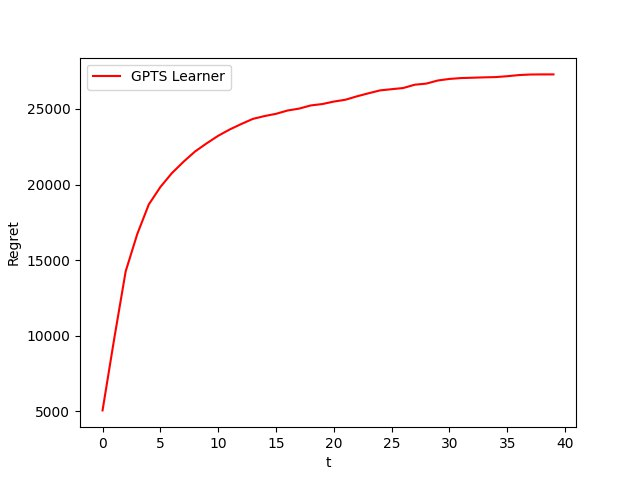
\includegraphics[width=1\textwidth]{../curves/results/budgetallocation_stationary_results}}
	
	\subsection{Sliding-Window Combinatorial Bandit Algorithm}
	\subsection{Learning Algorithm for Pricing}
	In this section, we describe the learning algorithm that we used to maximize the number of purchases made by users that have reached our website by clicking on ads.

\subsubsection{Assumptions}
\begin{enumerate}
    \item There is only one phase
    \item The allocation of the budget over the three subcampaigns is fixed
\end{enumerate}

\subsubsection{Setup of the experiment}
3 Thompson Sampling learners are used, one for each class of users. Since the users arrive on the purchase page by clicking on the ads, we assume that we can differentiate them by their class, thus proposing a different price to each user.

To satisfy assumption (1), the algorithm runs for a limited number of days, 45, enough to provide a significant result.

The average number of users that arrive per day are taken from the results of the previous point, which optimizes the budget in the fourth phase and maximizes the number of clicks. It returns the following average number of daily clicks: $C=[1800, 12000, 350]$. For this experiment, we will use these values as the daily average number of clicks, with a variance that is proportional to each value: $Var_i = C_i / 4$ $\forall{i} \in \{1,2,3\}$.

Since the optimization of the budget is made once a day and depends on the price chosen, also the price (for each class of users) is chosen once per day.

The minimum and maximum prices (0, 400) are the same for all the classes of users. The same goes for the number of arms, for which we tested various configurations ranging from 4 to 10 arms to see which one provided the best result.

\subsubsection{The algorithm}
The high-level pseudo code of the algorithm is shown in Algorithm \ref{alg:ts_pricing}.

Each TS learner is responsible for a class of users. Each day, the 3 learners pull the best price from their beta distributions. The prices are then proposed to all the users that arrive to the website on that day after clicking on the ads. At the end of the day, the learners are updated with the number of successes (purchases) for each class.

\begin{algorithm}
    \caption{TS learners for pricing}
    \label{alg:ts_pricing}
	\begin{algorithmic}[1]
        \STATE $J\gets ${ all classes of users}
        \STATE $T\gets ${ 45 days }
        \STATE $regret\gets ${0}
        \FOR{$day \in T $}
		\FOR{$j \in \{1,...,J\}$}
		\STATE $price\gets ${Draw a price from the j-th TS learner}
        \STATE $successes\gets ${number of buys with pulled price}
        \STATE $failures\gets ${clicks[j][day] - successes}
        \STATE $reward\gets ${successes * price}
        \STATE regret += optimum - reward
        \STATE TS[j].update(pulledArm, successes, failures)
        \ENDFOR
        \ENDFOR
	\end{algorithmic}
\end{algorithm}

Some remarks:
\begin{itemize}
    \item on line 6, to draw a price means that for each arm $a$ we pull a sample $\theta_a$ from the beta distribution, and then return the price $p_a$ of the arm that offers the best reward, that is $p_a = \underset{p_a}{argmax} \{p_a * \theta_a\}$
    \item on line 11 the update of the TS learner consists in updating the beta parameters of the arm pulled, in the following way: $(\alpha, \beta) += (successes, failures)$
\end{itemize}

\subsubsection{Choice of the best arm}
The following results come from averaging over 1000 experiments.

We tested the experiment with several numbers of arms. For each number $n$ of arms, draw the $n$ prices equally spaced in the interval and run the experiment, calculate the regret and the reward and use them to choose the best number of arms.

The first image shows the cumulative regret using different arms, ranging from 3 to 7.
Given the limited time-span, the best result is provided by a low number of arms, which converges more rapidly to the best arm.

However, since in the calculus of the regret we use as clairvoyant the best possible arm, we know how fast the learner converges but not how much money we would be losing in the ideal case in which we could use an infinite number of arms. For this reason, we set up another experiment in which we calculate the reward and compare it with the clairvoyant reward that, in this case, corresponds with the reward that we would get if we chose, for each class, its actual best price.

\begin{figure}[]
    \centering
    
    \caption{Reward of the TS Learner}
    \label{Reward of the TS Learner}
\end{figure}

As the image shows, using 3 arms does not offer a good reward. The best number of arms that comes out from our experiment is 4, which is aligned with the theoretical expection that we have with a period of 45 days.

\subsubsection{Results}
With 4 arms, we have a reasonably fast convergence to the best arm and enough arms to pull a price that is close enough to the clairvoyant to obtain a good reward.
	\subsection{Context Generator Algorithm}
	\subsection{Optimization Algorithm}
	\subsection{Optimization Algortihm Constrained}
\end{document}